\input{preamble.tex}

\NewBibliographyString{langjapanese}
\NewBibliographyString{fromjapanese}

\begin{document}

\Annot

Системы верификации --- программы, разработанные для формализации доказательств на компьютере. Б\'{о}льшая часть из них базируется на теории типов, которая делится на множество подвидов.
Гомотопическая теория типов (Homotopy type theory, HoTT) выделяется тем, что основывается на связи между теорией типов и теорией гомотопий. Эта область лежит в основе Унивалентных оснований математики (Univalent Foundation, UF) --- попытки формализовать математику, используя в качестве фундамента не множества, а гомотопические типы или $\infty$-группоиды, а также высшие индуктивные типы (Higher Inductive Types, HIT). Этот подход интересен тем, что позволяет работать с гомотопической теорией, используя синтетический метод, то есть, не опираясь на более базовые примитивы, как, например, множества.

В данный момент существует несколько систем верификации, которые поддерживают гомотопическую теорию типов нативно или благодаря расширениям, но эта поддержка обеспечивается различными наборами примитивных операций, для некоторых из которых существует совсем мало примеров.
В работе рассматривается формализация нетривиального расслоения над окружностью --- ленты Мёбиуса, а также портирование доказательства изоморфизма тривиальных расслоений и зависимых типов на верификатор доказательств Arend. Это доказательство показывает, что базовые теоретико-типовые конструкции соответствуют гомотопическим.

Код, которому посвящена данная работа, можно найти на GitHub\autocite{Grp1} в репозитории организации Groupoid Infinity. Доказательство выполнено в файле Fiber.ard\autocite{Fiber}, формализация ленты Мёбиуса --- в файле Moebius.ard\autocite{Moebius}.

\Introduction

Proof assistants are computer systems, which are designed to do mathematics on a computer. Some proof assistants also allow to define functions and compute on them, but their main focus is on doing proofs. They allow to define some statements and to reason about their correctness. A few of them, which are also automated theorem provers, also help a user with a set of well-chosen decision procedures that allow to automatically prove formulas of a specific restricted format\autocite{ProofAssistants1}.

A large part of proof assistants is based on type theory, which is due to Curry–Howard correspondence---correspondence between logical and type-theoretic operations. There are a few classifications of type theories. One of these classifications divides type theories between two flavors: \textit{intensional type theories} and \textit{extensional type theories}. The former is the flavor in which types that represent equalities are not necessarily propositions. Type theory, which is not intensional, is called extensional. The following work was performed with one of the flavors of intensional type theory---homotopy type theory, which takes seriously the natural interpretation of identity types as formalizing path space objects in homotopy theory. This type theory comes with a few benefits: higher inductive types, which help to obtain quotients objects or free structures, univalence that simplifies the process of moving back and forth between isomorphic structures, and a synthetic approach to homotopy theory.

There are several proof assistants, which support homotopy type theory natively or via extensions. Some of them are Coq\autocite{Coq}, Agda\autocite{Agda}, cubicaltt\autocite{Cubicaltt}, and redtt\autocite{Redtt}. They come with different sets of most basic operations. Some of these sets are studied better than others. Arend\autocite{Arend} is a proof assistant, which provides users with an interval type (a type that is inductively constructed from two terms, whose interpretation is as the endpoints of the interval, together with a path between them); an eliminator for an interval type---\textit{coe}, which allows, for every type over the interval, to transport elements from the fiber over left to the fiber over an arbitrary point; a dependent path type, which consists of all functions that maps elements of the interval type to the term of type parameterized by the given term of the interval type; and a function \textit{iso}, which can be used to define univalence---one of the cornerstones of homotopy type theory\autocite{Arenddocs}\autocite{nlab}.

Homotopy type theory relies on the idea that type-theoretic constructions correspond to some equivalents from homotopy theory. E.g., the statement that the term $a$ is of type $A$, which is written as $a:A$, can be expressed as ``$A$ is a space and $a$ is a point of A''. In addition to the kinds of types and terms above, we also may consider types and terms with parameters. These are usually called \textit{dependent} types (or \textit{family of types}) and terms (if $B$ is a type, then we might have a type $(x:B)\ E(x)$, which is parameterized by $B$). From the homotopy-theoretic point of view, we might think of such a type as a \textit{fibration} $E \to B$ over the space $B$. The fibration makes precise the idea of one space (\textit{fiber}) being parameterized by another (\textit{base}) with fibers being equivalent in some coherent way.

In this paper I report on formalizing a Moebius strip and on porting a proof of equivalence of the fibration and the family of types using the proof assistant Arend. The former task is a demonstration of basic Arend features and the latter is an evidence of correspondence between basic constructions of homotopy theory and type theory. The code can be found in Arend Groupoid Infinity repository (moebius strip: Moebius.ard\autocite{Moebius}, proof: Fiber.ard\autocite{Fiber}).

\section{Preliminaries}

Type theory contains two basic judgments. The first, typing judgment $a : A$, states that a term $a$ has type $A$. The motivation behind this notion varies:
\begin{enumerate}
	\item $a$ is an element of set $A$.
	\item $A$ is a problem and $a$ is a solution of $A$.
	\item $a$ is a proof of a proposition $A$.
	\item $A$ is a space and $a$ is a point of $A$.
\end{enumerate}
The first perspective is due to Russell, the second is due to Kolmogorov, the third is due to Curry and Howard and the fourth alternative comes from homotopy type theory\autocite{Warren1}. 
The second judgment, $a \equiv b : A$, asserts, that terms $a$ and $b$ are judgementally equal at type $A$. Judgemental equality is a relation between linguistic expressions and can be used to rewrite expressions\autocite{hottbook}. A notion of assumption is present in type theories in the form of type-context.
A definition of the type-context depends on the concrete theory. For the following definitions, it can be thought of as any finite set of judgments. E.g. $\Gamma = \{a : A, b : A, c : C\}$. The turnstile $\vdash$ between a context and a type judgment should be interpreted as: ``in the context $\Gamma$, the expression $a$ has type $A$''. E.g. $\Gamma \vdash a : A$. The rules of type theory tell us how to construct new types, how to construct terms of some types, and how to use such terms to construct terms of other types. The rules can be written as follows:
\begin{prooftree}
\AxiomC{$\Gamma \vdash f : A \to B$}
\AxiomC{$\Gamma \vdash a : A$}
\BinaryInfC{$\Gamma \vdash f(a) : B$}
\end{prooftree}
This rule states that given terms $f : A \to B$ and $a : A$ in the context of $\Gamma$ we can derive a term $f(a) : B$.
Also we can construct dependent types. Dependent types can be defined using a few postulates\autocite{Wellen1}:
\begin{enumerate}
  \item A Russell style hierarchy of type universes (types whose terms are types) is given: $U_0, U_1, U_2, \dots$. The hierarchy is cumulative: $U_m : U_n$ for $m < n$, and also if $A : U_m$ and $m \leq n$, then $A : U_m$. With universes, we can write the judgment ``$A$ is a type'' as a judgment that $A$ is a term of some universe. The HoTT book uses this approach.  
  \item If the universe level is unambiguous, then the level may be dropped to reduce unnecessary information.
  \item For any types $A$ and $B$, we may form a type $A \to B$ that represents a function. And a term $f : A \to B$ of this type may be constructed by demonstrating that $f(a) : B$ under the assumption $a : A$.
  \item A dependent type is a morphism to the universe $P : A \to U$, so a dependent type $P : A \to U$ provides us with a type $P(a)$ for any $a : A$. A judgment $x : A \vdash B(x) : U$ is a dependent type over $A$.
\end{enumerate}

Now let's turn to several of the constructions more closely related to the homotopy-theoretic side of things. Fibrations can be understood as a homotopy-theoretic generalization of the notion of a fiber bundle. If working with spaces, a fibration is a map $\phi : E \to B$, which possesses a certain homotopy-lifting property. In this particular case, we would refer to $B$ as the \textit{base space} and to $E$ as the \textit{total space} of the fibration. Given a point $b : B$, the \textit{fiber} over $b$ is just preimage $\phi^{-1}(b)$ of $b$ under the map $\phi$. The idea behind the fibration that it can be completely recovered from its base space $B$ together with its fibers by ``connecting'' the fibers together in accordance with the structure of the base space. Let's proceed with a more formal definition\autocite{Warren1}.
The homotopy fiber of a morphism $f : E \to B$ over a point of $B$ is the collection of elements of $E$ that are mapped by $f$ to this point, hence it is the following pullback (or fiber product) of $pt$ ($\star$-valued point of $B$) and $f$:

\[
\begin{diagram}
	\node{E \times \star}
		\arrow{s,t}{}
		\arrow{e,t}{}
	\node{\star} 
		\arrow{s,r}{pt} \\
	\node{E}
		\arrow{e,r}{f} 
	\node{B}
\end{diagram}
\]

Let's call fibration any continuous map $p : E \to B$, which has the homotopy-lifting property from arbitrary spaces. $E$ will be called the total space and $B$ the base space of the fibration. There are a lot of different fibrations, which come with restriction to this general definition (e.g. trivial fibration, Serre fibration, and so on)\autocite{Warren1}.

A fibration $\phi$ is trivial if it is equivalent to a product fibration\autocite{Warren1}.

\[
\begin{diagram}
	\node{E}
		\arrow{s,t}{\phi}
		\arrow{e,t}{f}
	\node{B' \times F} 
		\arrow{s,r}{proj_{B'}} \\
	\node{B}
		\arrow{e,r}{\hat{f}} 
	\node{B'}
\end{diagram}
\]
    
Two fibrations over a circle with fiber given by the unit interval $[0,1]$ are the cylinder and the Moebius strip, they are visualized in Figure \ref{fig:1}.

\begin{figure}[H]
\centering
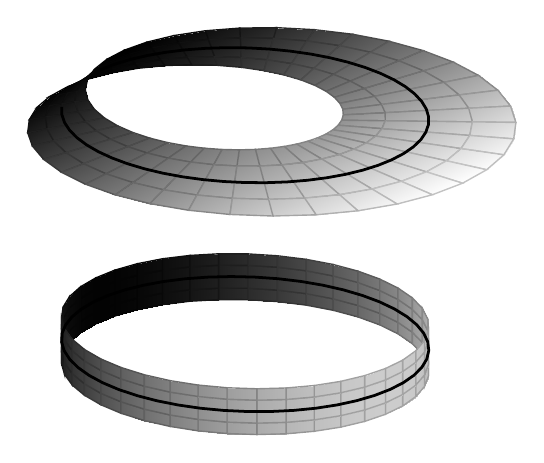
\begin{tikzpicture}[scale=1.25]
\begin{axis}[
    hide axis,
    view={40}{30}
]
\addplot3 [
    surf, shader = faceted interp,
    point meta = x,
    colormap/blackwhite,
    samples = 40,
    samples y = 5,
    z buffer = sort,
    domain = 0:360,
    y domain = -2:2
] (
    {sin(x)},
    {cos(x)},
    {y-20}
  );
  
\addplot3 [
    samples = 50,
    domain = 0:360,
    samples y = 0,
    thick
] (
    {cos(x)},
    {sin(x)},
    {-20}
  );   
  
\addplot3 [
    surf, shader = faceted interp,
    point meta = x,
    colormap/blackwhite,
    samples = 40,
    samples y = 5,
    z buffer = sort,
    domain = 0:360,
    y domain = -1:1
] (
    {(1+0.5*y*cos(0.5*x)))*cos(x)},
    {(1+0.5*y*cos(0.5*x)))*sin(x)},
    {0.5*y*sin(0.5*x)}
  );
  
\addplot3 [
    samples = 50,
    domain = -145:180,
    samples y = 0,
    thick
] (
    {cos(x)},
    {sin(x)},
    {0}
  ); 
\end{axis}
\end{tikzpicture}
\caption{Fibrations over a circle} \label{fig:1}
\end{figure}

\section{Moebius strip as an example of a fibration}

Now, let's start with an example of combining fibrations and dependent types---formalizing Moebius strip using Arend proof-assistant.
Intuitively, we need to find a way to encode a twist that distinguishes the Moebius strip from the cylinder. Since the fiber is the interval, our goal is to ``rotate'' it. In order to do so we can get a path induced by a map that rotates interval using univalence. 
 
\begin{ListingEnv}[H]
\begin{lstlisting}
\func neg_neg : \Pi (x : I) -> ((inv seg) @ (inv seg @ x)) = x 
  => \lam x 
    =>  ((\lam x 
      => (\lam i 
        => inv (connAnd (inv seg) i)) (inv seg @ x)) x)
        # (inv ((\lam x 
          => ((\lam x 
            => (\lam i 
              => inv (connAnd seg i)) (seg @ x)) x) # seg) x))

\func twist : I = I => Iso=>Path
    \new Iso I I neg neg neg_neg neg_neg
\end{lstlisting}
\end{ListingEnv}

Actually, \texttt{inv seg @ i} can be seen as $1-i$, so the function defined above shows that for an arbitrary interval point $i$ and for an arbitrary path $p$ $(-p)\ @\ (1-i)\ =\ i$.

Now we are able to ``continuously'' get a twisted interval for every term of type $S_1$, which represents a circle.

\begin{ListingEnv}[H]
\begin{lstlisting}
\func M : \Pi (x : S1) -> \Type => \lam x => \case x \with {
  | base => I
  | loop i => twist @ i
}
\end{lstlisting}
\end{ListingEnv}

The element $base : S_1$ is mapped to the interval type and other elements of $S_1$ are mapped to the elements, obtained using the path \texttt{twist}.

Finally, we can obtain a formalization of the Moebius strip as the total space of a nontrivial fibration over the circle. 

\begin{ListingEnv}[H]
\begin{lstlisting}
\record Moebius (p1 : S1) {
  \field f1 : M(p1)
}
\end{lstlisting}
\end{ListingEnv}

The projection map, which returns the first element of this dependent pair, is a fibration, $S_1$ is a base, and fibers are given by function \texttt{M}.

\section{Isomorphism between a fibration and a dependent type}

To prove a correspondence between the fibration and the dependent type we need to formalize these two notions, to provide mutually inverse functions between these constructions and to prove that homotopies between compositions of these two functions and identity functions exist. 
A formalization of a dependent type is straightforward---it is a function that maps elements of some type to types.

\begin{ListingEnv}[H]
\begin{lstlisting}
\func family (B : \Type) : \Type => B -> \Type
\end{lstlisting}
\end{ListingEnv}

Now let's define the total space of a fibration $B \to U$.

\begin{ListingEnv}[H]
\begin{lstlisting}
\func total (B : \Type) (F : family B) : \Type 
	=> \Sigma (x : B) (F x)
\end{lstlisting}
\end{ListingEnv}

Also we need to define a projection that will serve as a trivial fibration.

\begin{ListingEnv}[H]
\begin{lstlisting}
\func trivial (B : \Type) (F : family B) : total B F -> B 
	=> \lam (x : total B F) => x.1
\end{lstlisting}
\end{ListingEnv}

The homotopy fiber of $f : A \to B$ over $base : B$ can be defined as an element of $A$ together with a path from $f x$ to $base$.

\begin{ListingEnv}[H]
\begin{lstlisting}
\func fiber (A B : \Type) (f : A -> B) (base : B)
   => \Sigma (x : A) (f x = base)
\end{lstlisting}
\end{ListingEnv}

Now we need to define mutually inverse functions between the type that represents a family of types and the type that represents a trivial fibration. 
  
\begin{ListingEnv}[H]
\begin{lstlisting}
\func encode (B : \Type) (F : B -> \Type) (y : B) :
      fiber (total B F) B (trivial B F) y -> F y
   => \lam (x : fiber (total B F) B (trivial B F) y)
   => subst B F x.1.1 y x.2 x.1.2
\end{lstlisting}
\end{ListingEnv}

To construct an element of a given dependent type parameterized by some element $y : B$ from the fiber of trivial projection over the same element we can use a wrapper around an eliminator for the interval type. The function \texttt{subst} transports $u : P\ x$ to $P\ y$ along $p : x = y$.

An inverse of the previous function can be defined by straightforward construction.

\begin{ListingEnv}[H]
\begin{lstlisting}
\func decode (B : \Type) (F : B -> \Type) (y : B) :
      F y -> fiber (total B F) B (trivial B F) y
   => \lam (x : F y) => ((y, x), path (\lam i => y))
\end{lstlisting}
\end{ListingEnv}

Since \texttt{trivial} is just a projection, we can define a path for a fibration as a constant path.

To prove that a composition of decode and encode in this particular order is just an identity map we can prove that application of some element $x$ to the composition equals the exactly same element.

\begin{ListingEnv}[H]
\begin{lstlisting}
\func decode->encode (B : \Type) (F : family B) (y : B) :
  \Pi (x : F y) -> (encode B F y (decode B F y x)) = x
  => \lam (x : F y)
    => path (\lam i
      => encode
              B
              F
              y
              (decode B F y x))
\end{lstlisting}
\end{ListingEnv}

Since the outer function has an extra computational rule because it is defined with coe, the needed function can be defined as a constant path.

The second homotopy is harder to define. We need to define three paths---one for each element of a given fibration. The first path is trivial but the other two come with some difficulties, since these paths connect elements of different types. The problem with the second path is illustrated in Figure \ref{fig:2}.

\begin{figure}[H]
\centering
\begin{tikzpicture}
\draw plot [smooth cycle] coordinates {(-0.83,-2.31)(-1.73,0.25)(-1.15,2.29)(1.07,1.60)(1.74,-1.93)(0.31,-2.62)} 
node at (0.25,-3) {$F\ y$};

\draw plot [smooth cycle] coordinates {(5.83,-2.31)(3.73,0.25)(3.15,2.29)(6.07,1.60)(6.74,-1.93)} 
node at (5.65,-3) {$F\ x.1.1$};

\coordinate (p1) at (-0.5,-1);
\node[above left=5pt of {p1}, outer sep=2pt] {$encode\ B\ F\ y\ x$};
\filldraw (p1) circle[radius=1.5pt];

\coordinate (p2) at (5.75,-1.52);
\node[above right=5pt of {p2}, outer sep=2pt] {$coe\ A\ a\ right$};
\filldraw (p2) circle[radius=1.5pt];

\coordinate (p3) at (4.22,1.44);
\node[above=5pt of {p3}, outer sep=2pt] {$x.1.2$};
\filldraw (p3) circle[radius=1.5pt];

\draw[-latex] (p1) to [bend left] node [sloped,midway,below=0.5cm]{$path (\lambda i\ =>\ coe\ A\ a\ i)$} (p2);

\draw[-latex] [densely dotted](p2) to [bend right] node [sloped,midway,above]{?} (p3);

\draw[-latex][densely dotted] (p1) to[bend left] node [sloped,midway,above right=0cm and 0.3cm]{$p$} (p3);
\end{tikzpicture}
\caption{}
\label{fig:2}
\end{figure}

Our goal is to define $p$. Since we can construct a path from $encode\ B\ F\ y\ x$ to $coe\ A\ a\ right$, we need to find a path from $coe\ A\ a\ right$ to $x.1.2$. This path is provided by \texttt{transport\_twist}.

The third path is obtained almost in the same way with some adjustments for paths.

\begin{ListingEnv}[H]
\begin{lstlisting}
\func encode->decode (B : \Type) (F : family B) (y : B) :
  \Pi (x : fiber (total B F) B (trivial B F) y)
    -> (decode B F y (encode B F y x)) = x
  => \lam (x : fiber (total B F) B (trivial B F) y)
    => path (\lam i
      => (((inv x.2) @ i,
           (pathOverFamily (transport_twist F x.2 x.1.2)) @ i),
          (pathOverFamily ((coe_path (inv x.2) rfl rfl)
                      # (comp-assoc (inv (inv x.2)) rfl rfl)
                         # (refl-right ((inv (inv x.2)) # rfl))
                            # (refl-right (inv (inv x.2)))
                               # (inv_inv x.2))) @ i))
          \where
            \func transport_twist {A : \Type} (B : A -> \Type)
                                  {a b : A}
                                  (p : a = b) (x : B a) :
              transport B (inv p) (transport B p x) = x
              => J (\lam z (p' : a = z)
                => transport B (inv p') (transport B p' x) = x) rfl p
\end{lstlisting}
\end{ListingEnv}

To obtain an element of the identity type \texttt{(fiber (total B F) B (trivial B F) y) = (F y)} from equivalence we can use an univalence. To do so we can use a wrapper around Arend built-in function iso that implies the univalence axiom.

\begin{ListingEnv}[H]
\begin{lstlisting}
\func hFiber=DependentTypeParameterized (B : \Type) 
	(F : family B) (y : B) : 
	(fiber (total B F) B (trivial B F) y) = (F y)
  => Iso=>Path 
  	(\new Iso 
  		(fiber (total B F) B (trivial B F) y) 
  		(F y) 
  		(encode B F y) 
  		(decode B F y) 
  		(encode->decode B F y) 
  		(decode->encode B F y))
\end{lstlisting}
\end{ListingEnv}

We can go even further. Since we have proved that for every element of base type \texttt{(fiber (total B F) B (trivial B F) y) = (F y)} holds, we can prove that family itself equals a fiber over an arbitrary point.

\begin{ListingEnv}[H]
\begin{lstlisting}
\func Fibration=DependentType (B : \Type) (F : family B) : 
  (fiber (total B F) B (trivial B F)) = F
  => path (\lam i y
    => (hFiber=DependentTypeParameterized B F y) @ i)
\end{lstlisting}
\end{ListingEnv}

\Conc

In this paper I provided the proof of correspondence between dependent types---basic type theoretic constructions, and fibrations---basic homotopy theoretic constructions in the proof-assistant Arend. This correspondence shows that working on homotopy theory can be approached syntactically if using type theory with ease, because there is no need for complex definitions of the simplest homotopy construction.

\begin{otherlanguage}{english}
\printbibliography[
    heading=bibintoc
    ,title=Bibliography
]
\end{otherlanguage}

\end{document}
